\documentclass{beamer}
\beamertemplatenavigationsymbolsempty
\usecolortheme{rose}
\setbeamertemplate{blocks}[rounded=true, shadow=true]
\setbeamertemplate{footline}[page number]
%
\usepackage[utf8]{inputenc}
\usepackage[english, russian]{babel}
\usepackage{amssymb,amsfonts,amsmath,mathtext}
\usepackage{subfig}
\usepackage{graphicx}
\usepackage[most]{tcolorbox}
\usepackage[all]{xy} % xy package for diagrams
\usepackage{array}
\usepackage[dvipsnames]{xcolor}
\usepackage{multicol}% many columns in slide
\usepackage{hyperref}% urls
\usepackage{multirow}
\usepackage{hhline}%tables
% Your figures are here:
\graphicspath{ {fig/} {../fig/} }
\usepackage{ragged2e}
\justifying
\documentclass{amsart}
\definecolor{skyblue}{rgb}{0.75, 0.87, 0.93}

%----------------------------------------------------------------------------------------------------------
\title{{Анализ неопределенности и внутренних представлений языковых моделей для поиска сгенерированных документов}}
\author{
    Анастасия Евгеньевна Вознюк\\
    Научный руководитель: к.ф.-м.н. А.\,В.\,Грабовой
}
\date{18 мая 2024 г.}
\institute[МФТИ (НИУ)]{
    Кафедра интеллектуальных систем ФПМИ МФТИ\\
    Специализация: Интеллектуальный анализ данных\\
    % Направление: 01.03.02 Прикладные математика и информатика\\
}
\date{\footnotesize
% \par\smallskip\emph{Научный руководитель:} Андрей Грабовой
\par\bigskip\small 21 декабря 2024}

%----------------------------------------------------------------------------------------------------------
\begin{document}
%----------------------------------------------------------------------------------------------------------
\begin{frame}
\thispagestyle{empty}
\maketitle
\end{frame}
%-----------------------------------------------------------------------------------------------------
\begin{frame}{Цель работы}

Исследуется проблема поиска сгенерированных документов. Стандартные методы поиска не являются устойчивыми к смене генератора или смене домена, поэтому нужно предложить более устойчивые методы.

Требуется предложить метод поиска сгенерированных фрагментов с помощью анализа неопределенности языковой модели, которой передан документ, требующий проверку. Помимо этого, предлагается исследовать методы анализа внутренних представлений языковых моделей, а также внутренних размерностей текстов при обработке текстового документа.



\end{frame}
%----------------------------------------------------------

\begin{frame}{Общая постановка задачи}
Определим документ как конечную последовательность символов из заданного алфавита $\mathbf{W}$. Пространство документов:
$$\mathbb{D} = \Bigl\{\Big[t_j\Big]_{j=1}^n \quad|\quad t_j \in \mathbf{W}, n \in \mathbb{N}\Bigr\}.$$

Дан набор из $N$ документов
$$\mathbf{D} = \bigcup_{i=1}^{N}D^i, D^i \in \mathbb{D}.$$

Определим множество авторов, тексты которых встречаются в наборе $\mathbf{D}$:
$$\mathbf{C} = \{0, \dots, k - 1\}.$$


Тогда задача классификации автора документа записывается как: 
\begin{equation}
    \mathbf{\phi}: \mathbb{D} \rightarrow \mathbf{C}
\end{equation}
\end{frame}

% \begin{frame}{Детекция фрагментов в документе}
% Для каждого документа $d \in \mathbb{D}$ существует представление в виде разбиения на фрагменты различного авторства:
% $$ \mathbb{T} = \Bigl\{\Big[t_{s_j}, t_{f_j}, C_j\Big]_{j = 1}^{J} \quad|\quad t_{s_j} = t_{f_{j - 1}},\quad s_j \in \mathbb{N}_0,\quad f_j \in \mathbb{N}, \quad C_j \in  \mathbf{C} \Bigr\},$$

% где $J$ - количество фрагментов разного авторства в документе, $t_{s_j}$ и $t_{f_j}$ - начало и конец $j$-ого фрагмента, внутри которого все токены одного авторства, $C_j$ - автор $j$-ого фрагмента. 

% \newline
% Тогда модель детектора определяется как композиция отображений:
% $$\mathbf{\phi}: \mathbb{D} \rightarrow \mathbb{T} \quad \quad \mathbf{\phi} : \mathbf{g} \circ \mathbf{f},$$
% где $\mathbf{f}$~--- отображение для выделения текстовых фрагментов, а $\mathbf{g}$  - отображение для классификации получившихся фрагментов.
% \end{frame}

\section{Uncertainty estimation}
\begin{frame}{Анализ неопределенности}

% Suggest we have our input context $\textbf{x}$, $y_k = f(\textbf{x}, y_1, \dots, y_{k - 1} |\textbf{\theta})$, $\textbf{y} = [y_1, \dots, y_n]^T$


$\pmb{\theta}$ - параметры нашей модели $f$. 
$$y_k = f(D, y_1, \dots, y_{k - 1} \mid \pmb{\theta})$$
$$\pmb{y} = [y_1, \dots, y_n]^T$$

\textbf{Maxiumum Sequence Probability}
\begin{equation}  
\text{MSP}(\pmb{y} | D, \pmb{\theta}) = 1 -P(\pmb{y} | D, \pmb{\theta})
\end{equation} 


\textbf{Perplexity}
\begin{equation}
P(\textbf{y} | D,  \pmb{\theta}) = \exp\{-\frac{1}{|D|}\log P(\textbf{y} | D, \pmb{\theta})\}
\end{equation} 

\textbf{Mean Token Entropy}
\begin{equation}
\mathcal{H}_T(\mathbf{y}, D ; \boldsymbol{\theta})=\frac{1}{|D|} \sum_{l=1}^{|D|} \mathcal{H}\left(y_l \mid \mathbf{y}_{<l}, D, \boldsymbol{\theta}\right)
\end{equation} 

\end{frame}


\begin{frame}{Вычислительный эксперимент}

% Было взято 1000 человеческих текстов и 1000 текстов 
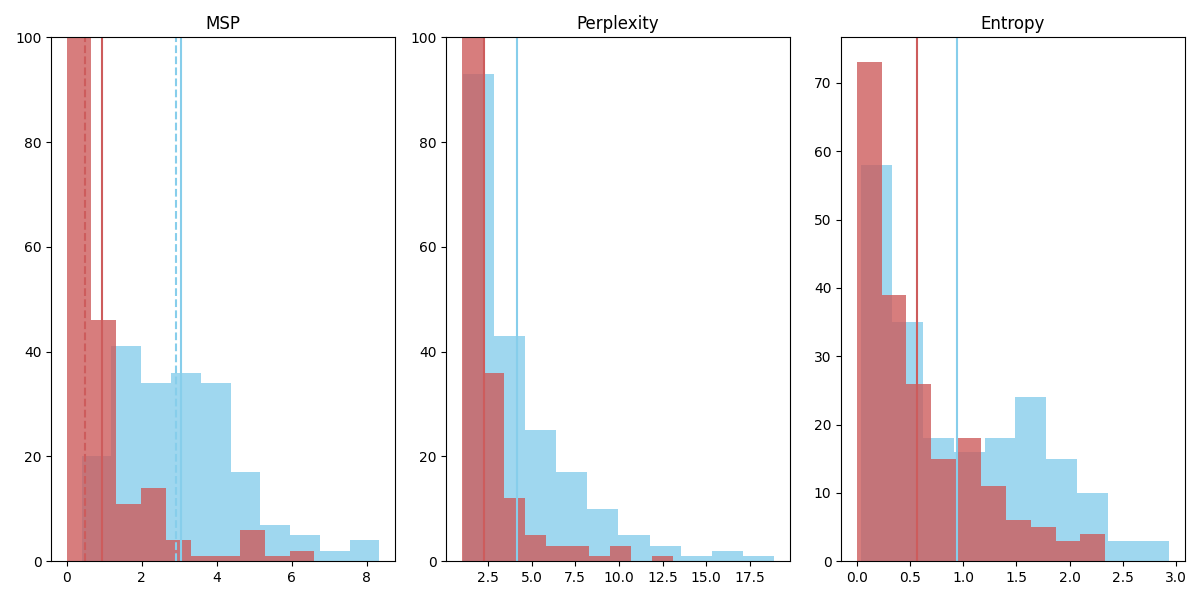
\includegraphics[width=\textwidth]{Surname2021PresentationSample/fig/metrics.png}
Было взято 1000 человеческих текстов и 1000 текстов и на них были посчитаны фнукции, описанные на предыдущем слайде: \textbf{Maximum Sequence Probability, Perplexity, Mean Token Entropy}.
    
\end{frame}

%--------------------------------------------------------------------
\section{PHD}
\begin{frame}{Использование топологических признаков текста}
    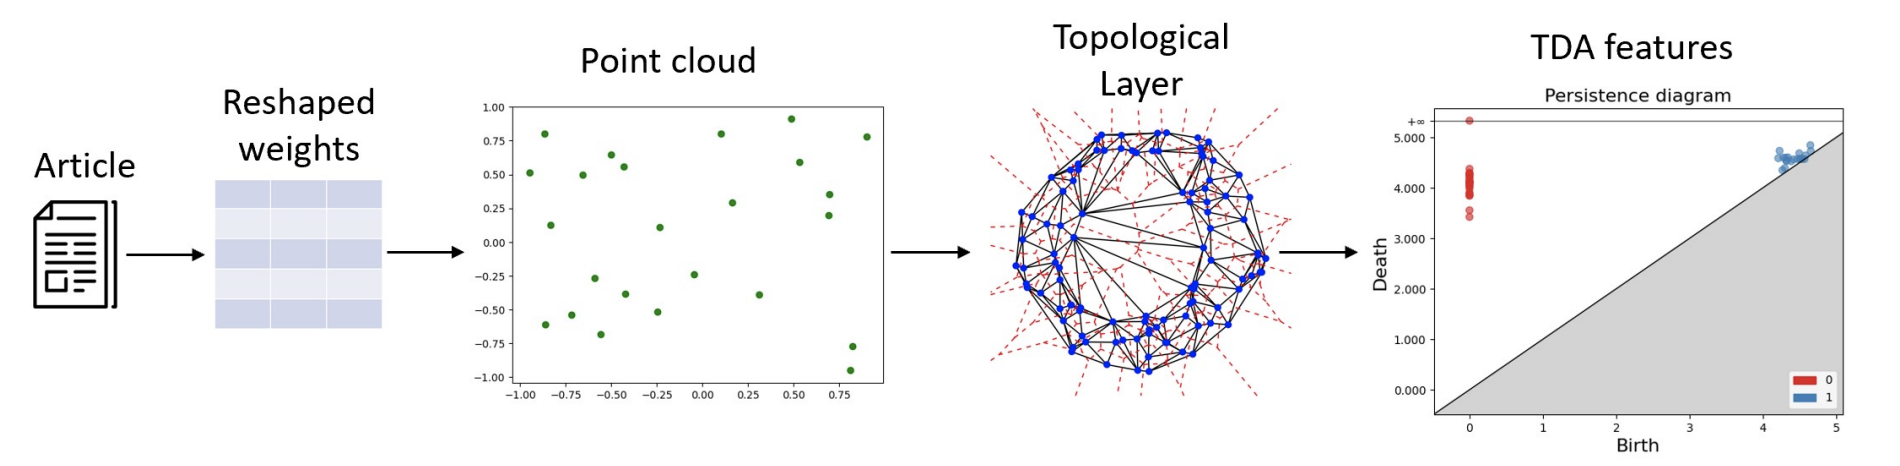
\includegraphics[width=\textwidth]{Surname2021PresentationSample/fig/topology_pipeline.png}

    Основной подход основан на использовании понятий персисентной гомологии конечного набора точек $\mathcal{M}$ в метрическом пространстве с метрикой $d$.

    $E_t = \{(v, u): v, u \in \mathcal{M}, \quad d(v, u) \leq t\} \quad \forall t \in (0, \infty)$

    Персисентная гомология $\text{PH}_i$ определена набором признаков размерности $i$, так $\text{PH}_0$ задается компонентами связности, $\text{PH}_1$ - циклами, и т.д. 
    

\end{frame}
%______________________________
\begin{frame}{Внутреняя размерность}
  У каждого признака есть своя \textit{продолжительность жизни}, это пара $(t_\text{birth}, t_\text{death})$, когда данный признак появляется, и когда исчезает.
  
Введем $\alpha$-взвешенную сумму, $I(\gamma)$ - продолжительность жизни признака $\gamma$.
\begin{equation}
    E_\alpha^i(X):=\sum_{\gamma \in \mathrm{PH}_i(X)}|I(\gamma)|^\alpha
\end{equation}

\begin{equation}
E_\alpha^0(X) \sim C n^{\frac{d-\alpha}{d}},  n\rightarrow \infty  \Leftrightarrow \alpha<d
\end{equation}

\begin{equation}
    \operatorname{dim}_{\mathrm{PH}}(\mathcal{M})=\inf \left\{d \mid \exists C \quad E_d^0(X) \leq C \quad \forall  X \subset \mathcal{M}, |X| < \infty \right\}.
\end{equation}

\begin{tcolorbox}[colback=white,colframe=skyblue,title=Гипотеза]
    Внутренняя размерность $\operatorname{dim}_{\mathrm{PH}}(\mathcal{M})$ показывает количество степеней свободы у точки в $\mathcal{M}$.
\end{tcolorbox}

\end{frame}

\begin{frame}{}
\textbf{Персисентная гомологическая размерность (PHD) } - метрика, основанная на внутренней размерности текстов, показала себя статистически значимой метрикой для разделения текстов разной природы для первых языковых моделей\footnote{Tulchinskii et al. Intrinsic Dimension Estimation for Robust Detection of AI-Generated Texts, NeurIPS 2023}. Однако для более новых моделей разделимость уже не такая хорошая.

% \begin{columns}[onlytextwidth]
%    \begin{column}{0.7\textwidth}
%       \centering
%       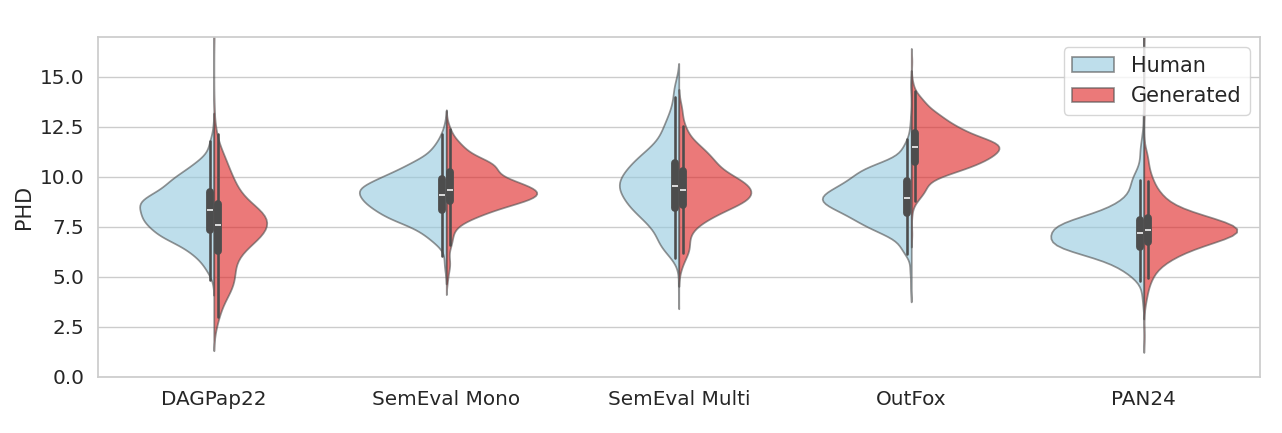
\includegraphics[width=200pt]{Surname2021PresentationSample/fig/violins_v2.png}% Place your graphic here
%     \end{column}
%     \begin{column}{0.3\textwidth}
%     Главная цель во время работы алгоритма - размещать "ядерные функции" $\mu_n$ в областях, где сосредоточена большая плотность вероятности
%     \end{column}
% ​  \end{columns}
% \end{frame}

\begin{tcolorbox}[colback=white,colframe=skyblue,title=Гипотеза]
    Можно адаптировать PHD для новых моделей, так что она все еще будет статистической метрикой разделимости текстов.
\end{tcolorbox}
\end{frame}

%--------------------------------------------------------------------
\begin{frame}{Вычислительный эксперимент}

\begin{table}
    \centering
    \begin{tabular}{l|c|c}
        Dataset & $\text{PHD}_{\text{human}}$ & $\text{PHD}_{\text{machine}}$ \\
        \hline
        OutFox & 8.96 $\pm$ 1.21 & 11.48 $\pm$ 1.13\\
        SemEval24 Mono & 9.11 $\pm$ 1.19 & 9.41 $\pm$ 1.2 \\
        SemEval24 Multi & 9.65 $\pm$ 1.81 & 9.42 $\pm$ 1.44  \\
         DAGPap22 & 8.35 $\pm$ 1.33 & 7.48 $\pm$ 2.01  \\
          PAN24 & 9.4 $\pm$ 1.05 & 8.52 $\pm$ 1.59  \\
          MGT-1 Mono & 9.19 $\pm$ 1.75 & 8.96 $\pm$ 2.24 \\
          MGT-1 Multi & 8.76 $\pm$ 1.85 & 8.6 $\pm$ 2.29 \\
    \hline    
    \end{tabular}
\end{table}


    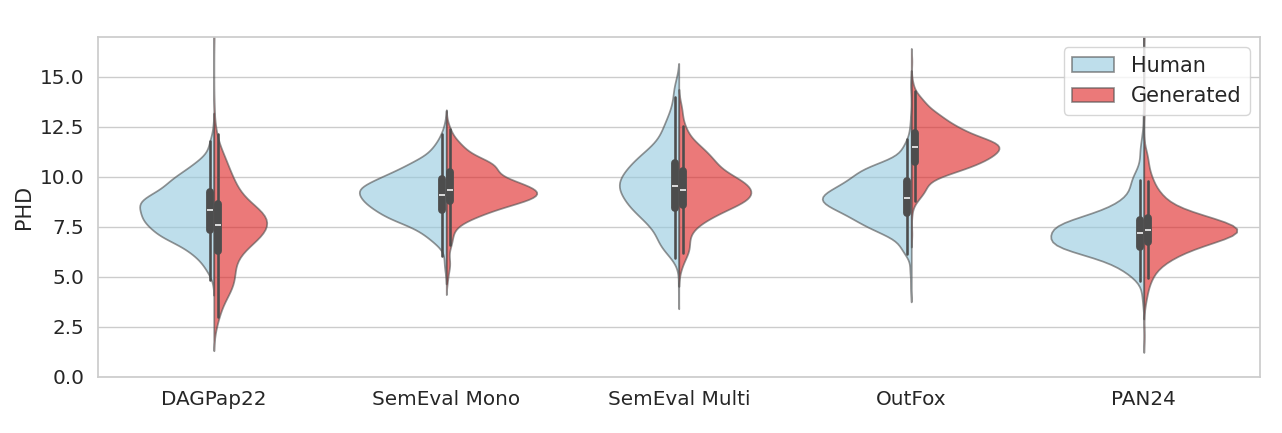
\includegraphics[width=\textwidth]{Surname2021PresentationSample/fig/violins_v2.png}
\end{frame}
%------------------------------------------------------------------------
\section{Анализ внутренних представлений}
\begin{frame}{Новый способ подсчитывать внимание}
    Пусть $N$ - длина текстовй последовательности. Выделим в тексте ''якоря`` $d_1, .., d_n$, в которых содержится основной смысл текста.  Рассмотрим голову внимания $h$ со слоя $l$ модели $M$. Определим \textit{QK-score} $S^{(l, h)}_{QK} (d_i)$ и \textit{Attention-score} $S^{(l, h)}_{Att} (d_i)$:
\begin{equation}
    S^{(l, h)}_{QK} (d_i) =  q_{N}^{(l, h) \top} k^{(l, h)}_{t_i},
    \quad 
    S^{(l, h)}_{Att} (d_i) =  a_{N, t_i}^{(l, h)},
    \quad 
    i \in \{1, 2,...,n\}
\end{equation}

\begin{tcolorbox}[colback=white,colframe=skyblue,title=Гипотеза]
    \textit{QK-score} может лучше решать задачу чем стандартный подсчет внимания и быть более интерпретируемым.
\end{tcolorbox}


\end{frame}

\begin{frame}{Вычислительный эксперимент}

    Данные два подхода подсчета внимания сравнивались на задаче ответов на тестовые вопросы MMLU.

\begin{table}[t]
    \centering
    \begin{tabular}{r|cccc}
        ~  & \multicolumn{4}{c}{\textbf{LLaMA...}} \\
        Method   & {\textbf{2-13B}} &  {\textbf{2-70B}} &  {\textbf{3-8B}} &  {\textbf{3-70B}} \\
        \hline
        Baseline, Acc  & 47.4 & 57.7 & 60.5 & \textbf{78.2}\\
        Baseline, PA & 34.6 & 45.9 & 47.7 & \textbf{70.1}\\
        QK-score, Acc & \textbf{49.7} & \textbf{58.9} & \textbf{63.0} & 77.9\\
        QK-score, PA & \textbf{38.3} & \textbf{47.1} & \textbf{49.3} & 67.9 \\
    \end{tabular}
    \caption{Сравнение различных моделей на датасете MMLU. Приводятся следующие метрики: Accuracy (Acc) и Permutation Accuracy ({PA)}.}
\end{table}

Дополнительно сравниваются другие датасеты с тестовыми вопросами, а также другие модели. Больше результатов приведено в статье.      
\end{frame}

\begin{frame}{Пример сравнения QK-Score и внимания}
    \texttt{What singer appeared in the 1992 baseball film 'A League of Their Own'$\backslash$nOptions:$\backslash$n}
    
    \texttt{A. Brandy.$\backslash$n}
    \texttt{B. Madonna.$\backslash$n}
    
    \texttt{C. Garth Brooks.$\backslash$n}
    \texttt{D. Whitney Houston.$\backslash$n}

    
    \texttt{E. I don't know.$\backslash$n}
    \texttt{F. None of the above.$\backslash$n}
    \begin{figure}
                \centering
                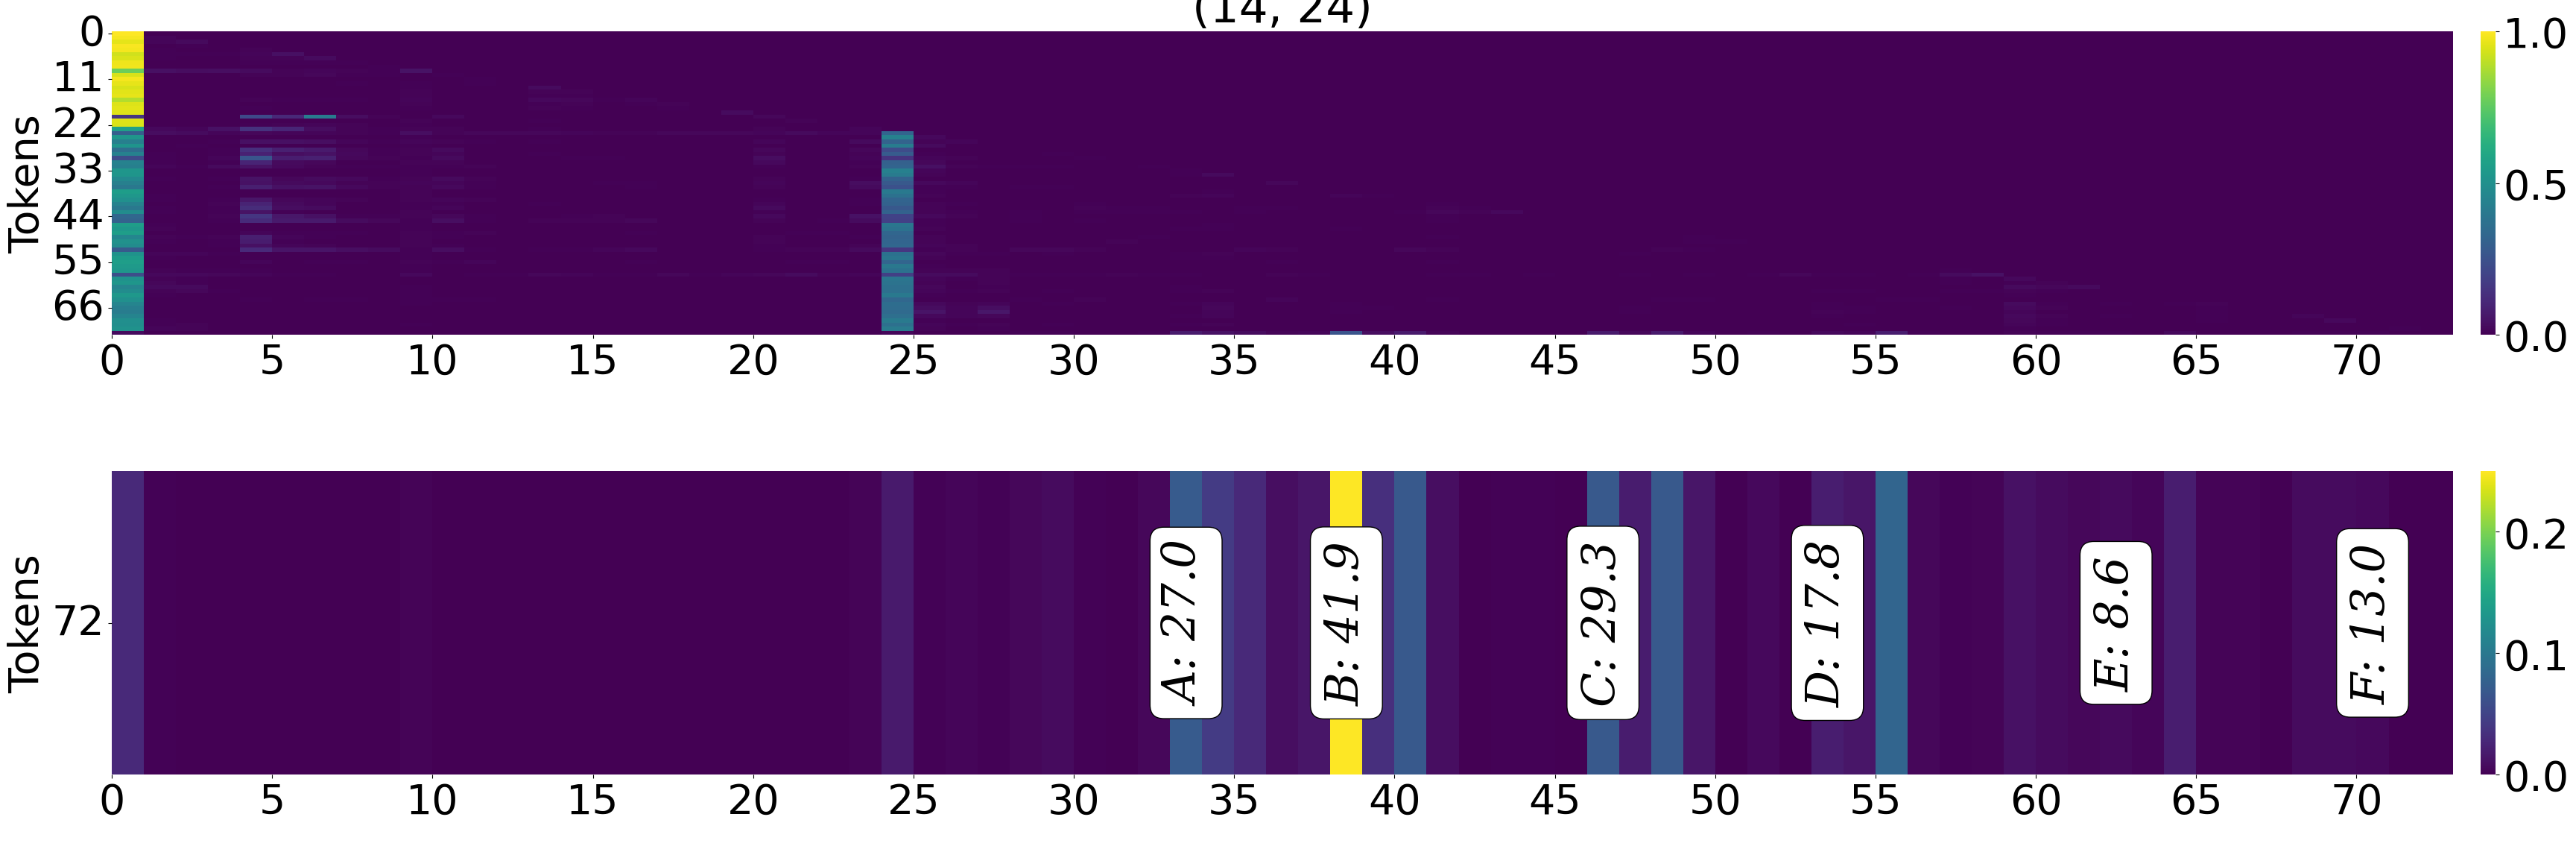
\includegraphics[width=\textwidth]{Surname2021PresentationSample/fig/attention_1.png} 
                \caption{Пример когда QK-Score и внимание выдают одинаковый ответ}
    \end{figure}
\end{frame}

\begin{frame}{Пример сравнения QK-Score и внимания}
     \texttt{What singer appeared in the 1992 baseball film 'A League of Their Own'$\backslash$nOptions:$\backslash$n}
    
    \texttt{A. Brandy.$\backslash$n}
    \texttt{B. Madonna.$\backslash$n}
    
    \texttt{C. Garth Brooks.$\backslash$n}
    \texttt{D. Whitney Houston.$\backslash$n}

    
    \texttt{E. I don't know.$\backslash$n}
    \texttt{F. None of the above.$\backslash$n}
    \begin{figure}
                \centering
                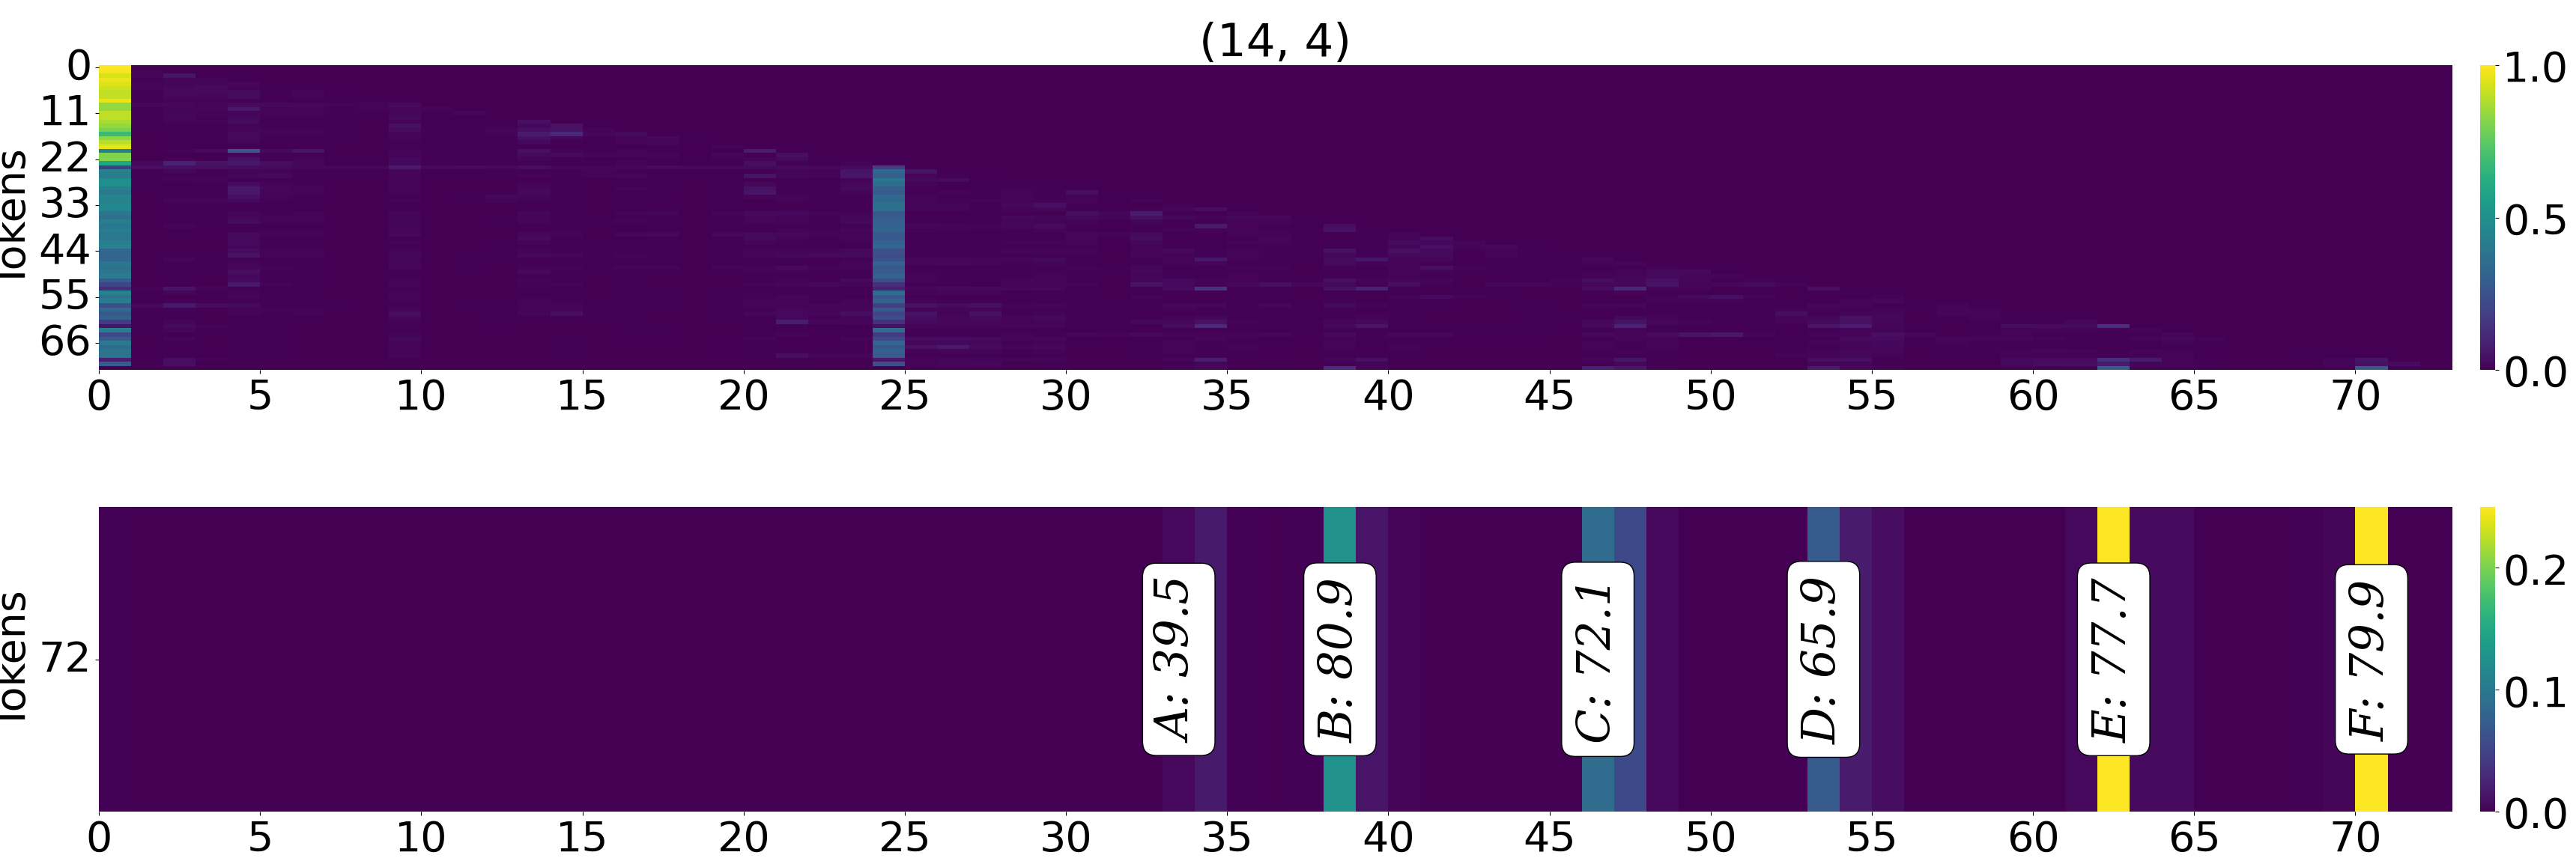
\includegraphics[width=\textwidth]{Surname2021PresentationSample/fig/attention_2.png} 
                \caption{Пример когда только QK-Score выдает корректный ответ}
    \end{figure}
\end{frame}

\section{итоги}
\begin{frame}{Итоги НИР за семестр и планы на следующий семестр}
    \begin{block}{Результаты}
    \begin{enumerate}
        \item Опубликована 1 работа на A* конференции, еще 1 принята к публикации, еще 2 в состоянии препринта и ожидают оценки ревьюеров;
        \item Получены первые результаты с анализом PHD для сгенерированных текстов и с оценкой неопределенности на них;
    \end{enumerate}
    \end{block}

    \begin{block}{Планы}
    \begin{enumerate}
        \item Предложить новые эксперименты для проверки гипотез;
        \item Необходимо модифицировать PHD чтобы добиться разделимости по текстам от более новых моделей;
        \item Модифицировать QK-Score для задачи поиска сгенерированных фрагментов, определить какие якоря могут быть в этой задаче;
    \end{enumerate}
    \end{block}
    
    % \begin{tcolorbox}[colback=white,colframe=skyblue,title=Планы]
    % Можно адаптировать PHD для новых моделей, так что она все еще будет статистической метрикой разделимости текстов.
    % \end{tcolorbox}
\end{frame}

%------------------------------------------------------------------------
% \begin{frame}{Выносится на защиту}
%     \begin{enumerate}
%         \item Архитектура решения для детекции смены авторов в текстах, когда смена авторов происходит только на уровне параграфов (результат осеннего семестра)
%         \item Архитектура решения для детекции смены авторов в тексте, в случае, когда эта смена авторов происходит единожды, но может быть в произвольном токене
%         \item Использование CRF для задачи детекции границ авторов
%     \end{enumerate}
% \end{frame}

\begin{frame}[noframenumbering,plain]{Список работ автора по теме НИР}
        \begin{block}{Публикации}
        \begin{enumerate}
            \item Listening to the Wise Few: Select-and-Copy Attention Heads for Multiple-Choice QA. \textit{arXiv preprint:2410.02343}
            \item Advacheck at GenAI Detection Task 1: AI Detection Powered by Domain-Aware Multi-Tasking, \textit{Proceedings of Workshop on Detecting AI Generated Content at COLING 2025}
            \item  Are AI Detectors Good Enough? A Survey on Quality of Datasets With Machine-Generated Texts, \textit{arXiv preprint:2410.14677}
        \end{enumerate}
    \end{block}
    \begin{block}{Выступления с докладом}
        \begin{enumerate}
            \item DeepPavlov 1.0: Your Gateway to Advanced NLP Models Backed by Transformers and Transfer Learning.// \textit{EMNLP, Miami, Florida}
        \end{enumerate}
    \end{block}
\end{frame}
%------------------------------------------------------------------------
\end{document} 